\documentclass{beamer}

\usepackage{graphicx,hyperref,url}
\usepackage[utf8]{inputenc}
\usepackage[T1]{fontenc}
\usepackage{booktabs}
\usepackage[portuges]{babel}
\usepackage{lmodern, comment}
\usepackage{xcolor}
\usepackage{pifont}
\usepackage[final]{listings}
%%\usepackage{udesc} 

%%% FIGS \graphicspath{{figures/}{../figures/}{C:/Users/me/Documents/project/figures/}}

\graphicspath{ {figures/} {../ia_combinatoria/figures/} }
%%%%\graphicspath{ {/home/user} }
\definecolor{azulclaro}{rgb}{0.9,0.9,0.9}
\definecolor{mygreen}{rgb}{0,0.6,0}
\definecolor{mygray}{rgb}{0.5,0.5,0.5}
\definecolor{mymauve}{rgb}{0.58,0,0.82}
\definecolor{darkgray}{rgb}{.4,.4,.4}
\definecolor{purple}{rgb}{0.65, 0.12, 0.82}


\lstset{ 
  %  label={pgm_ex01},
    backgroundcolor=\color{azulclaro}, 
    language=Haskell, %%Miranda,%%Perl,%%%Python, %%Mercury,
    showstringspaces=false,
    basicstyle=\bf\scriptsize\ttfamily,
%%      basicstyle= \footnotesize %%% TESTAR
%%      keywordstyle=\bfseries\color{green!40!black},
    keywordstyle=\textbf{\color{mygreen}}, 
    otherkeywords={*, \%, array, constraint, solve, output,  show, "/\", satisfy, set, of, if, then, elseif, float, search},
%%  keywordstyle=\color{blue},       % keyword style
%%    commentstyle=\itshape\color{purple!40!black},
      commentstyle=\color{orange},    % comment style
      identifierstyle=\color{blue},
      stringstyle=\color{orange},
      stringstyle=\color{mymauve},
      numbers=left,  % where to put the line-numbers; possible values are (none, left, right)
      numbersep=5pt,   % how far the line-numbers are from the code
      numberstyle=\tiny\color{magenta},
      keepspaces=true      
    % %caption={LEGENDA no source PASCAL ficou OK},
}



\title[Inteligência Artificial -- Otimização Combinatória] % (optional, use only with long paper titlebg=blue!20!white,s)
{Caminho Mínimo: \\ Uma Modelagem com\\ Programação Linear\\ Parte -- 01}

%\subtitle
%{About some things}

\author[Claudio Cesar de Sá] % (optional, use only with lots of authors)
{Claudio Cesar de Sá\inst{1}}
% - Give the names in the same order as the appear in the paper.
% - Use the \inst{?} command only if the authors have different
%   affiliation.

\institute[UDESC]{Pesquisador Independente}
%  Departamento de Ciência da Computação -- DCC\\
%  Centro de Ciências Tecnológicas -- CCT\\
% Universidade do Estado de Santa Catarina -- UDESC

% - Use the \inst command only if there are several affiliations.
% - Keep it simple, no one is interested in your street address.

\date[\today] % (optional, should be abbreviation of conference name)


\begin{document}

\begin{frame}
  \titlepage
\end{frame}



% Structuring a talk is a difficult task and the following structure
% may not be suitable. Here are some rules that apply for this
% solution: 

% - Exactly two or three sections (other than the summary).
% - At *most* three subsections per section.
% - Talk about 30s to 2min per frame. So there should be between about
%   15 and 30 frames, all told.

% - A conference audience is likely to know very little of what you
%   are going to talk about. So *simplify*!
% - In a 20min talk, getting the main ideas across is hard
%   enough. Leave out details, even if it means being less precise than
%   you think necessary.
% - If you omit details that are vital to the proof/implementation,
%   just say so once. Everybody will be happy with that.

%%%%%%%%%%%%%%%%%%%%%%%%%%%%%%%%%%%%%%%%%%%%%%%%%%%%%%%


\begin{frame}

\begin{block}{Roteiro}
%  \tableofcontents

\begin{enumerate}

  \item  Complexidade de Problemas
  \item O que é a Programação Linear Inteira (PLI)
  \item  Um problema:  Caminho Mínimo
  \item  Modelagem com uma técnica de PLI  $\Rightarrow$ \textbf{\textcolor{green}{este vídeo}}
  \item  Implementação e código com OR-TOOLS (Python) $\Rightarrow$  \textbf{\textcolor{red}{próximo vídeo}} 
  \item  Generalizando o Caminho Mínimo (avançado) $\Rightarrow$ \textbf{\textcolor{red}{um outro vídeo}} 
  \item Este material: \url{https://github.com/claudiosa/CCS/tree/master/presentations-seminars/cam_min_PL}
  \end{enumerate}

\end{block}

\end{frame}


%%%%%%%%%%%%%%%%%%%%%%%%%%%%%%%%%%%%%%%%%%%%%%%%%%%%%%%
\begin{comment}
\section{Para efeitos de TEMPLATE}
\begin{frame}
\frametitle{Nome do SLIDE}
\begin{block}{Nome do Bloco}
  \begin{itemize}
   \item T1

    \item<2-> T2

    \item<3-> T3

  \item<4-> 

    \item<5-> 
    
        \item<6-> 
    \end{itemize}
  
\end{block}

\end{frame}
\end{comment}
%%%%%%%%%%%%%%%%%%%%%%%%%%%%%%%%%%%%%%%%%%%%%%%%%%%%%%%

%%%%%%%%%%%%%%%%%%%%%%%%%%%%%%%%%%%%%%%%%%%%%%%%%%%%%%%%%
\section{Classes de Problemas}


\begin{frame}
\frametitle{Classes de Problemas}

\begin{figure}[ht!]
 \centering
 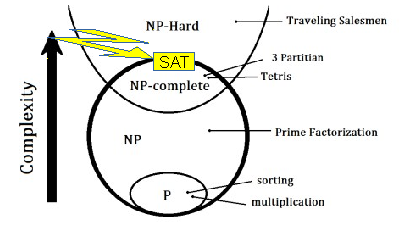
\includegraphics[width=0.8\textwidth , height=0.6\textheight]{classes_problemas.pdf}
 \caption{Alguns problemas e suas complexidades} 
%\label{}
\end{figure}

\end{frame}






%%%%%%%%%%%%%%%%%%%%%%%%%%%%%%%%%%%%%%%%%%%%%%%%%%%%%%%
\section{Programação Linear}
\begin{frame}
	\frametitle{Programação Linear}
	
	\begin{figure}[ht!]
		\centering
		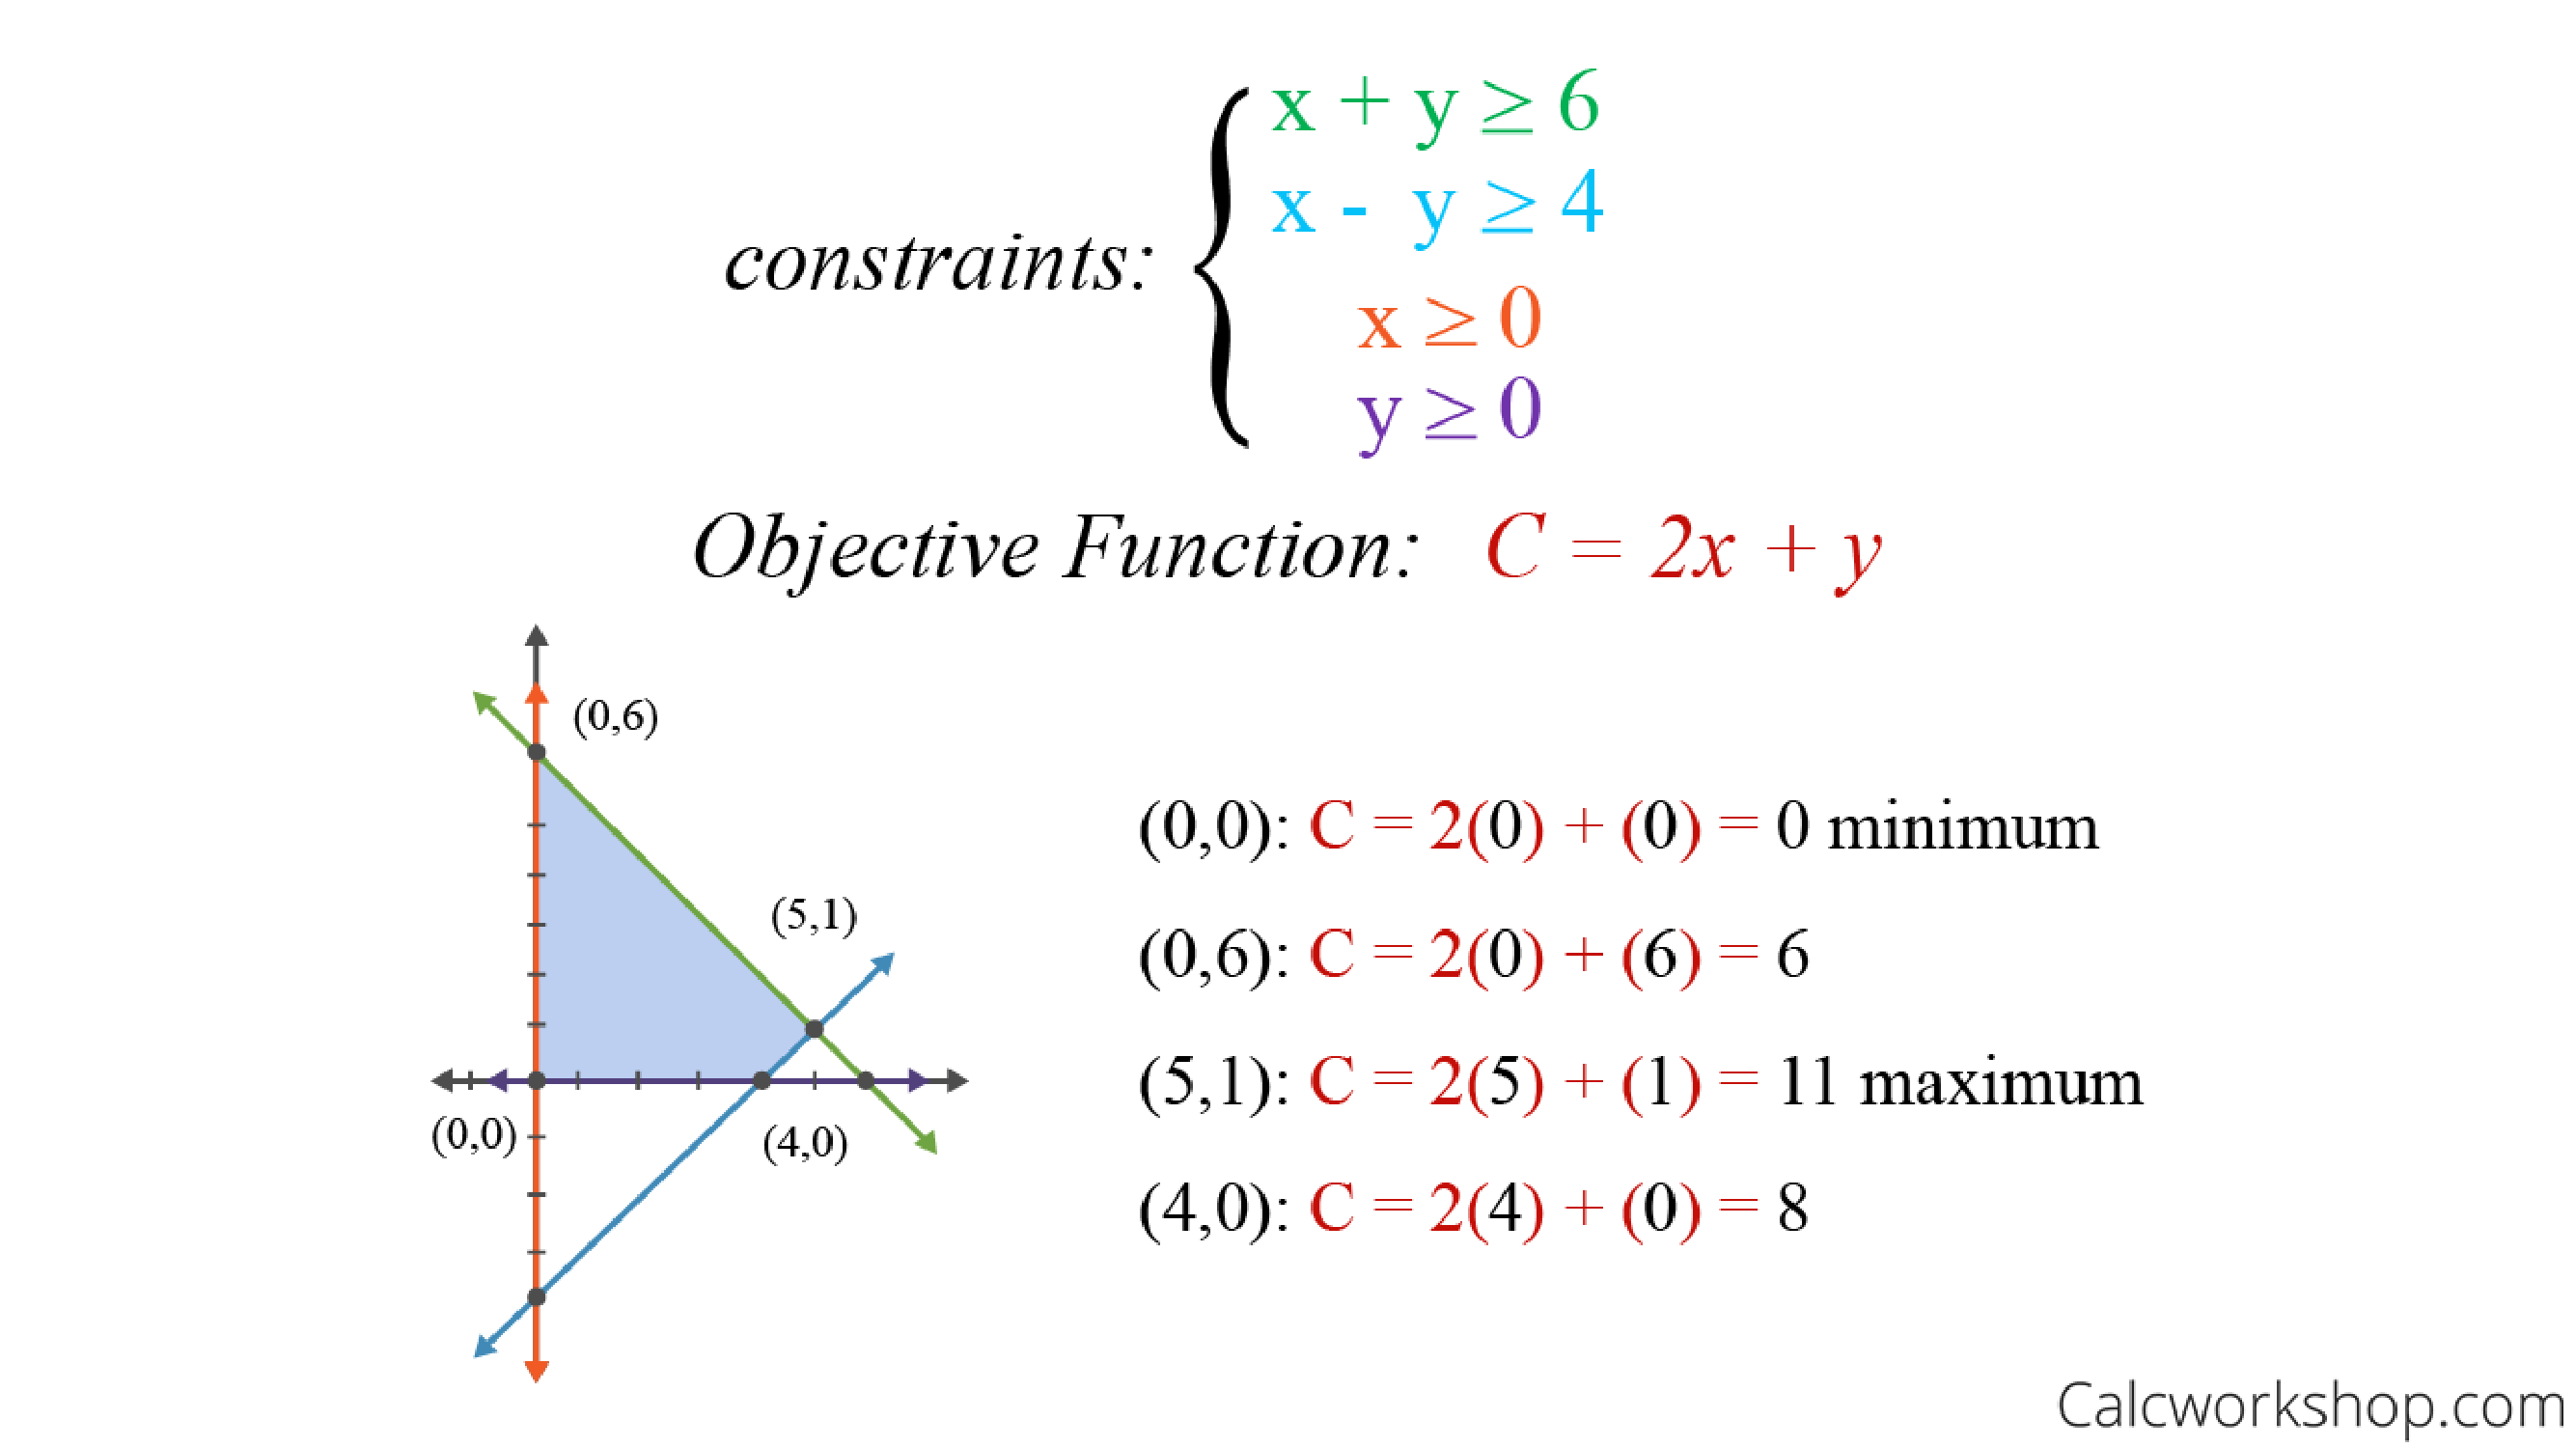
\includegraphics[width=0.9\textwidth , height=0.78\textheight]{linear-programming-example.pdf}
    	\caption{Uma técnica de resolver problemas: equações lineares} 
		%\label{}
	\end{figure}
	
\end{frame}


%%%%%%%%%%%%%%%%%%%%%%%%%%%%%%%%%%%%%%%%%%%%%%%%%%%%%%%
\section{Problema do Caminho Mínimo}

\begin{frame}
    \frametitle{Elementos de um Grafo}
    
    \begin{figure}[tbp]
     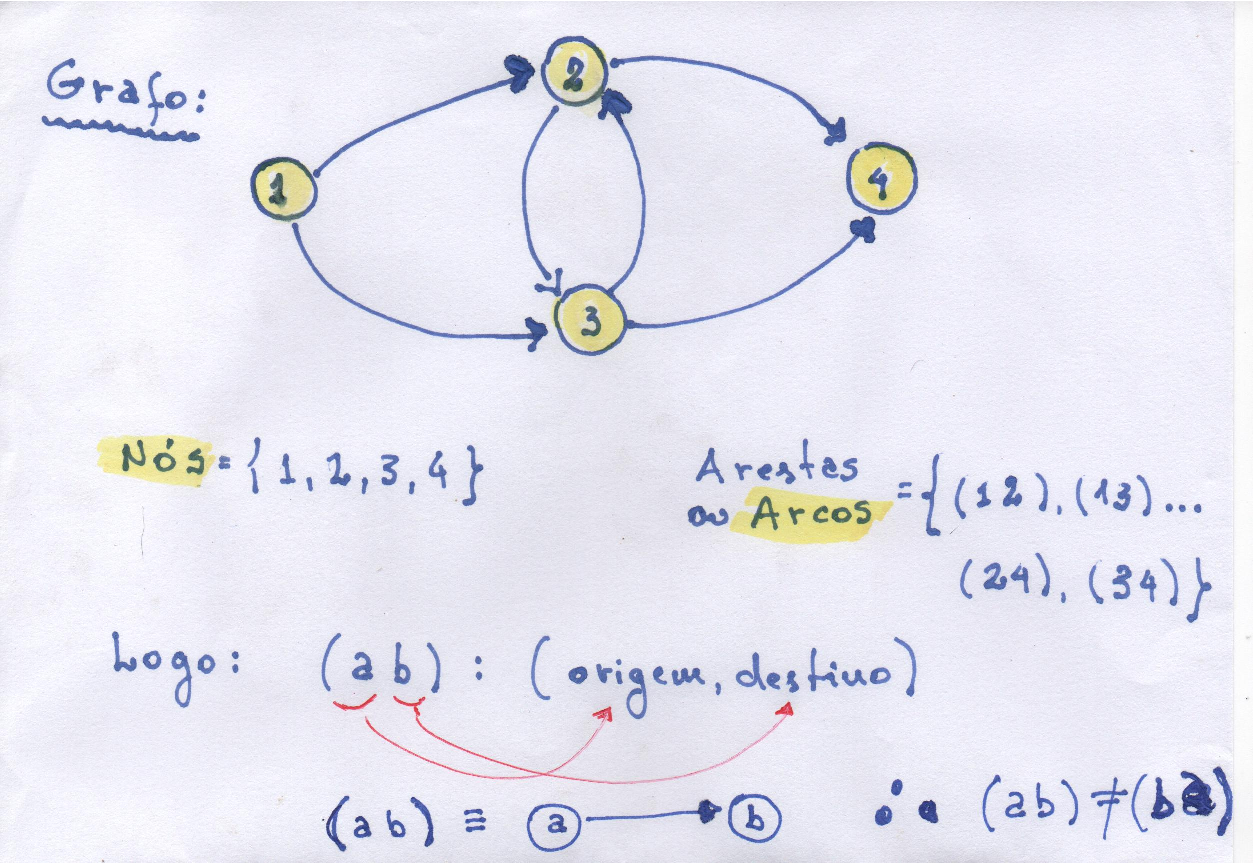
\includegraphics[keepaspectratio=true,width=0.8\textwidth , height=0.6\textheight]{01_elementos_de_um_grafo.pdf}
    \centering
    \end{figure}


\end{frame}
%%%%%%%%%%%%%%%%%%%%%%%%%%%%%%%%%%%%%%%%%%%%%%%%%%%%%%%
\begin{frame}
	\frametitle{Problema do Caminho Mínimo}
	
	\begin{figure}[tbp]
		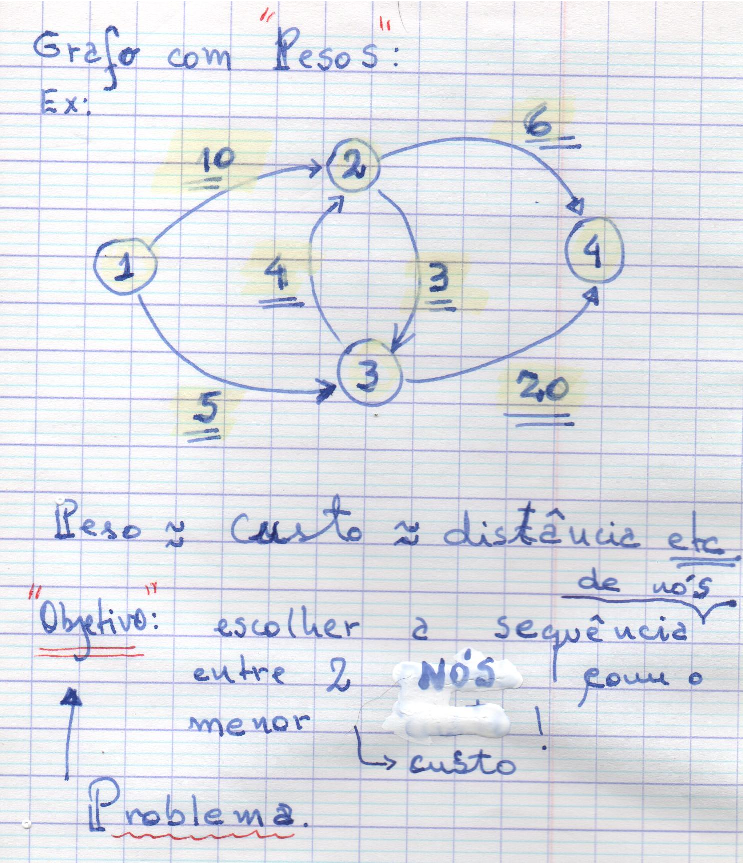
\includegraphics[width=0.8\textwidth , height=0.6\textheight]{02_grafo_com_pesos.pdf}
		\centering
		\caption{Um problema da classe P (mas muito útil) com uma solução via PLI}
	\end{figure}
Referência: \url{https://en.wikipedia.org/wiki/Shortest_path_problem}
\end{frame}
%%%%%%%%%%%%%%%%%%%%%%%%%%%%%%%%%%%%%%%%%%%%%%%%%%%%%%%


\begin{frame}
	\frametitle{Variável de Decisão e Uso}
	
	\begin{figure}[tbp]
		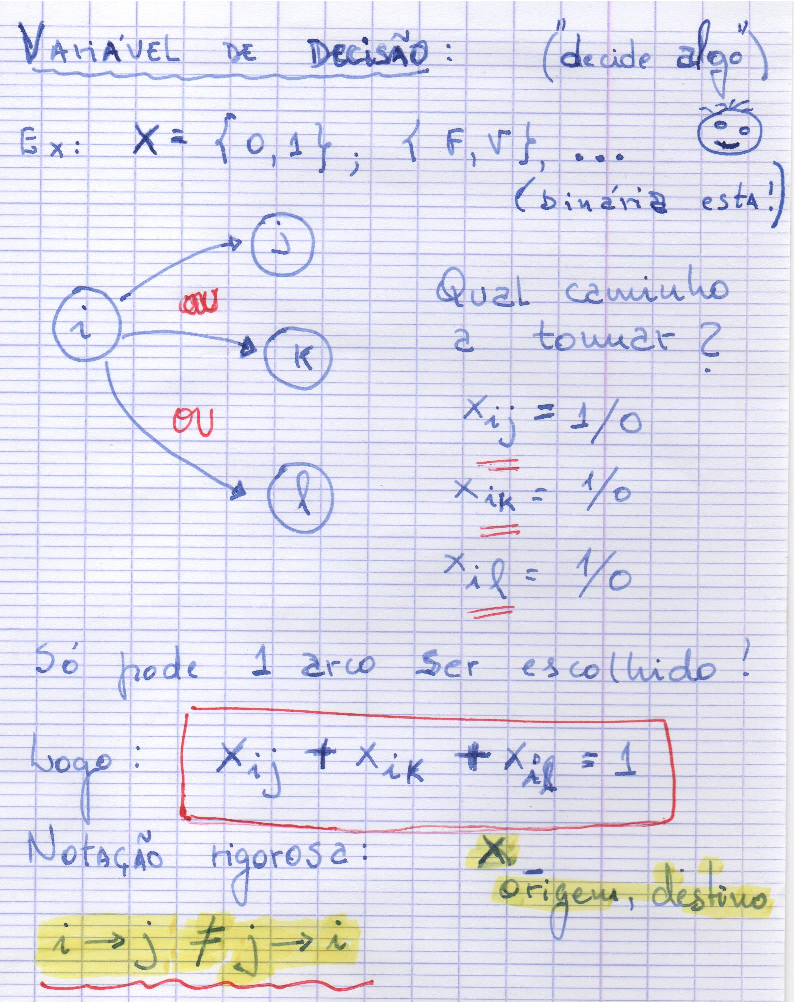
\includegraphics[width=0.8\textwidth , height=0.8\textheight]{03_variavel_decisao_uso.pdf}
		\centering
	\end{figure}
\end{frame}
%%%%%%%%%%%%%%%%%%%%%%%%%%%%%%%%%%%%%%%%%%%%%%%%%%%%%%%
\begin{frame}
	\frametitle{Matriz de Decisão e Uso}
	
	\begin{figure}[tbp]
		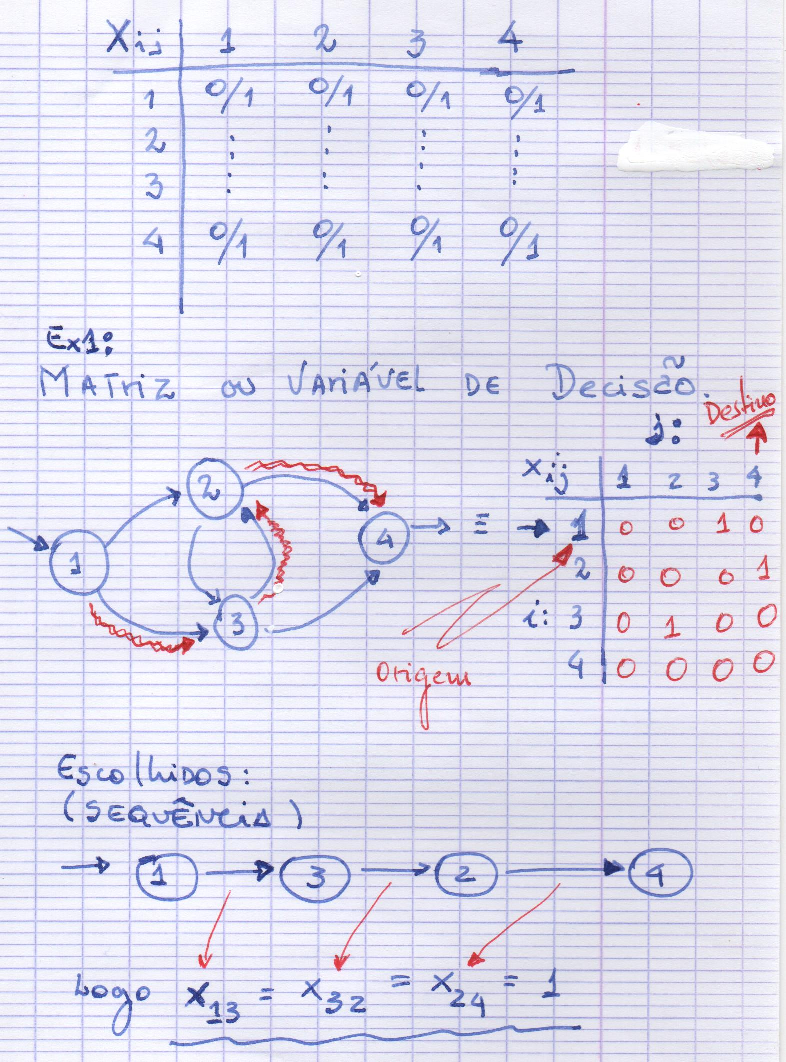
\includegraphics[width=0.8\textwidth , height=0.8\textheight]{04_matriz_decisao_uso.pdf}
		\centering
	\end{figure}
\end{frame}
%%%%%%%%%%%%%%%%%%%%%%%%%%%%%%%%%%%%%%%%%%%%%%%%%%%%%%%

\begin{frame}
	\frametitle{Definindo um Caminho}
	
	\begin{figure}[tbp]
		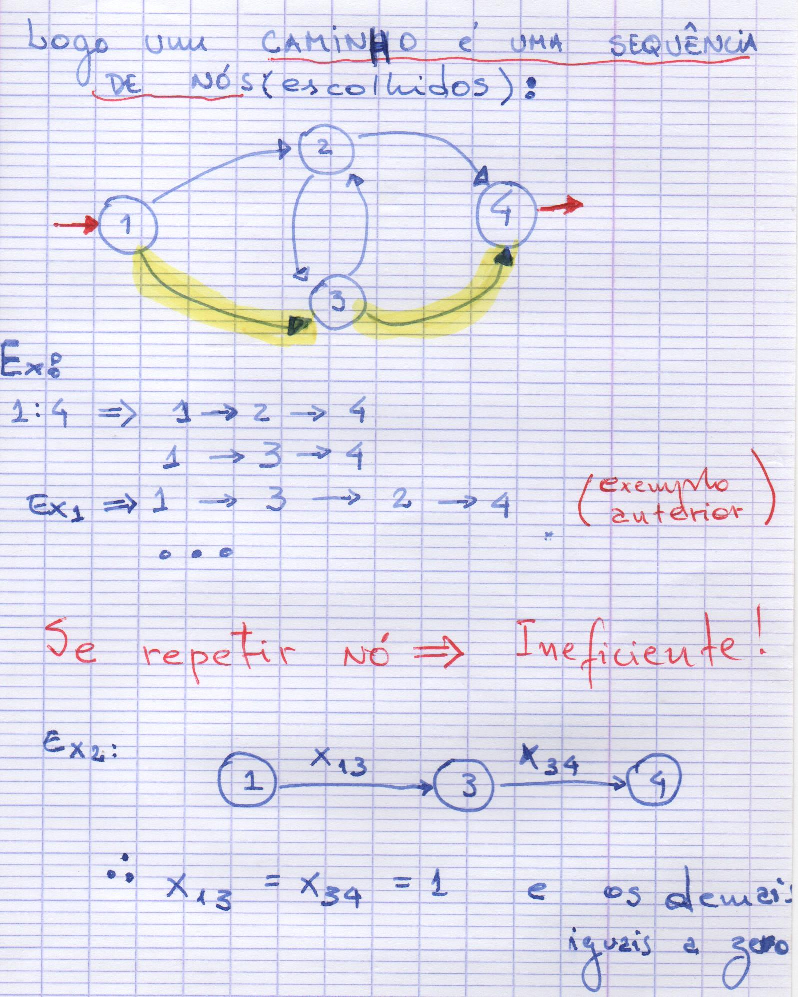
\includegraphics[width=0.8\textwidth , height=0.8\textheight]{05_um_caminho.pdf}
		\centering
	\end{figure}
\end{frame}
%%%%%%%%%%%%%%%%%%%%%%%%%%%%%%%%%%%%%%%%%%%%%%%%%%%%%%%


\begin{frame}
	\frametitle{O Caminho e a Matriz de Peso}
	
	\begin{figure}[tbp]
		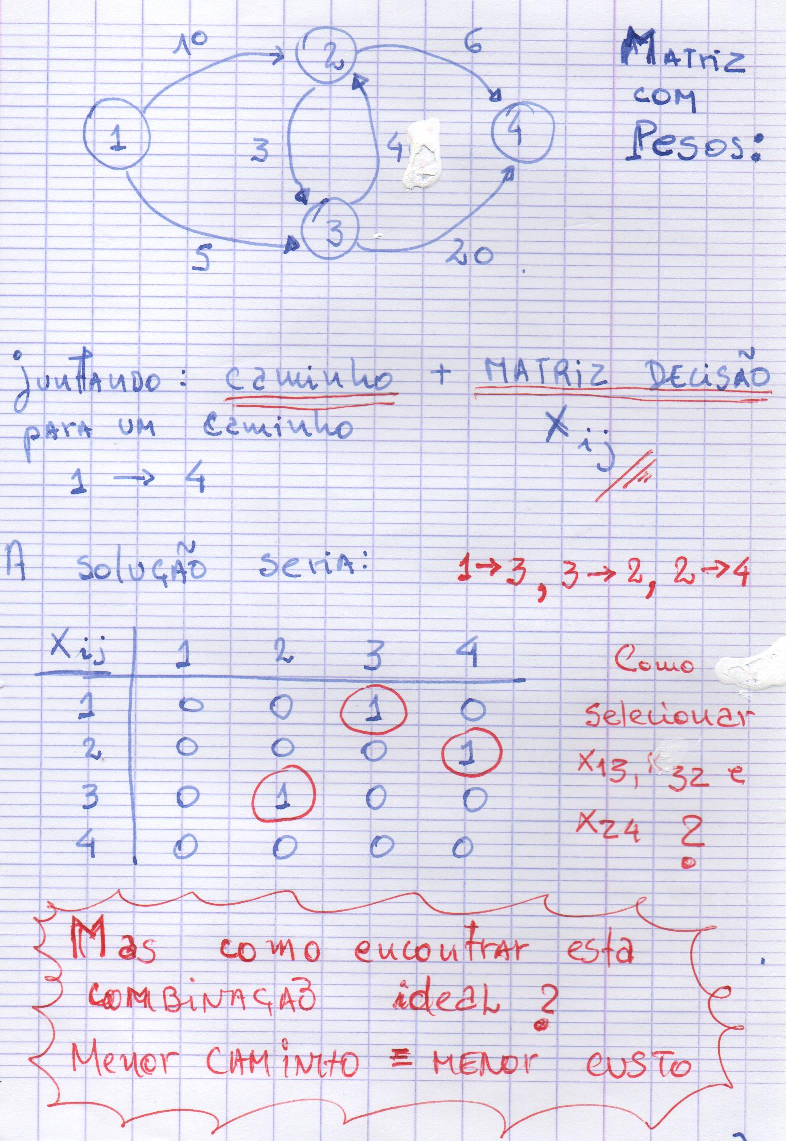
\includegraphics[width=0.8\textwidth , height=0.8\textheight]{06_um_caminho_e_matriz.pdf}
		\centering
	\end{figure}
\end{frame}
%%%%%%%%%%%%%%%%%%%%%%%%%%%%%%%%%%%%%%%%%%%%%%%%%%%%%%%

\begin{frame}
	\frametitle{Formalizando os Elementos}
	
	\begin{figure}[tbp]
		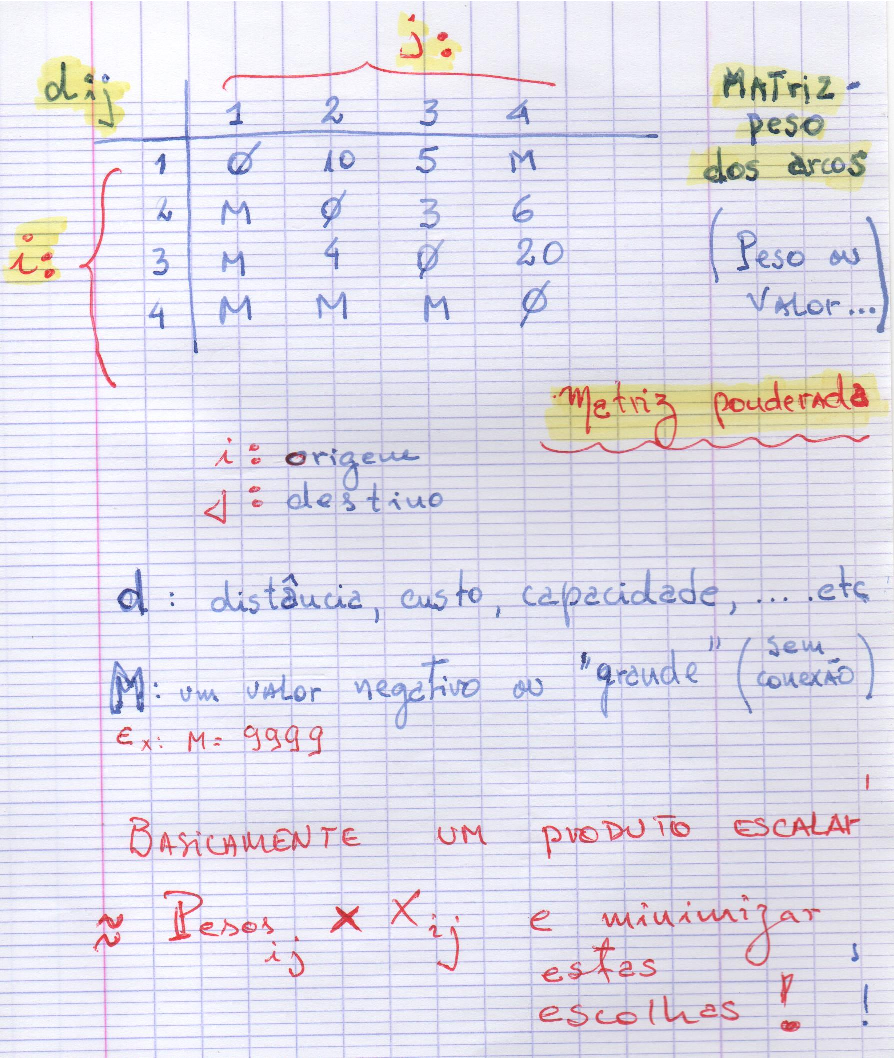
\includegraphics[width=0.8\textwidth , height=0.8\textheight]{07_formalizando.pdf}
		\centering
	\end{figure}
\end{frame}
%%%%%%%%%%%%%%%%%%%%%%%%%%%%%%%%%%%%%%%%%%%%%%%%%%%%%%%


\begin{frame}
	\frametitle{Estratégia deste Problema: {\bf Fluxo} ($\Phi$)}
	
	\begin{figure}[tbp]
		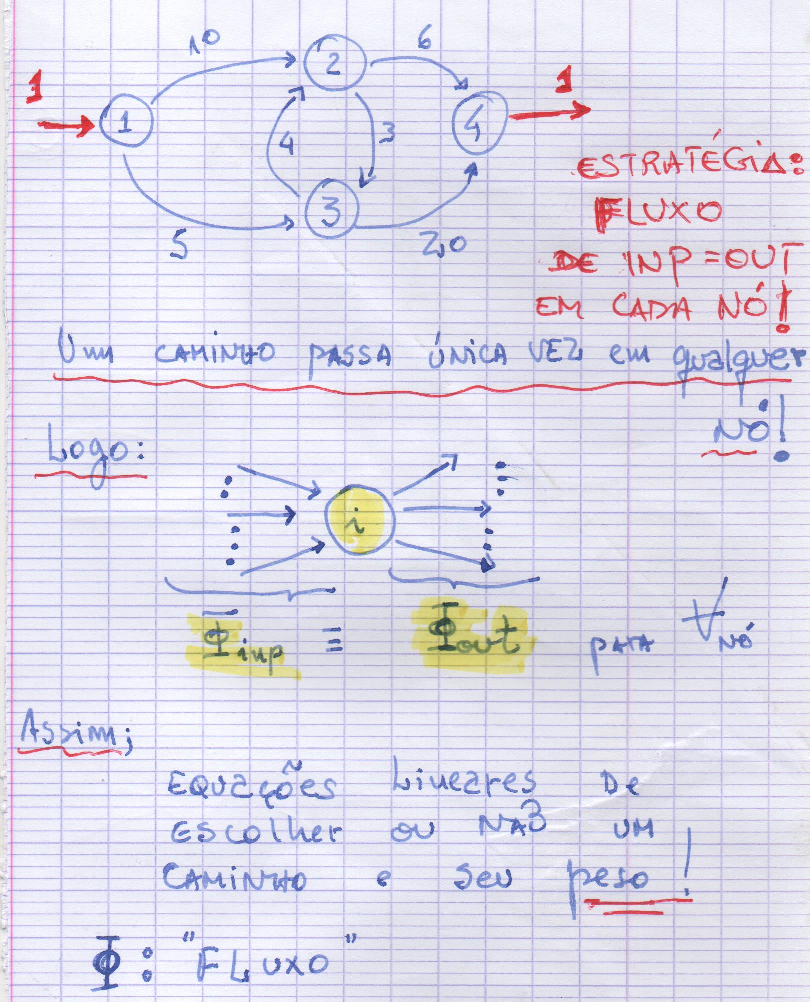
\includegraphics[width=0.8\textwidth , height=0.8\textheight]{08_fluxo_por_no.pdf}
		\centering
	\end{figure}
\end{frame}
%%%%%%%%%%%%%%%%%%%%%%%%%%%%%%%%%%%%%%%%%%%%%%%%%%%%%%%


\begin{frame}
	\frametitle{Equações Finais}
	
	\begin{figure}[tbp]
		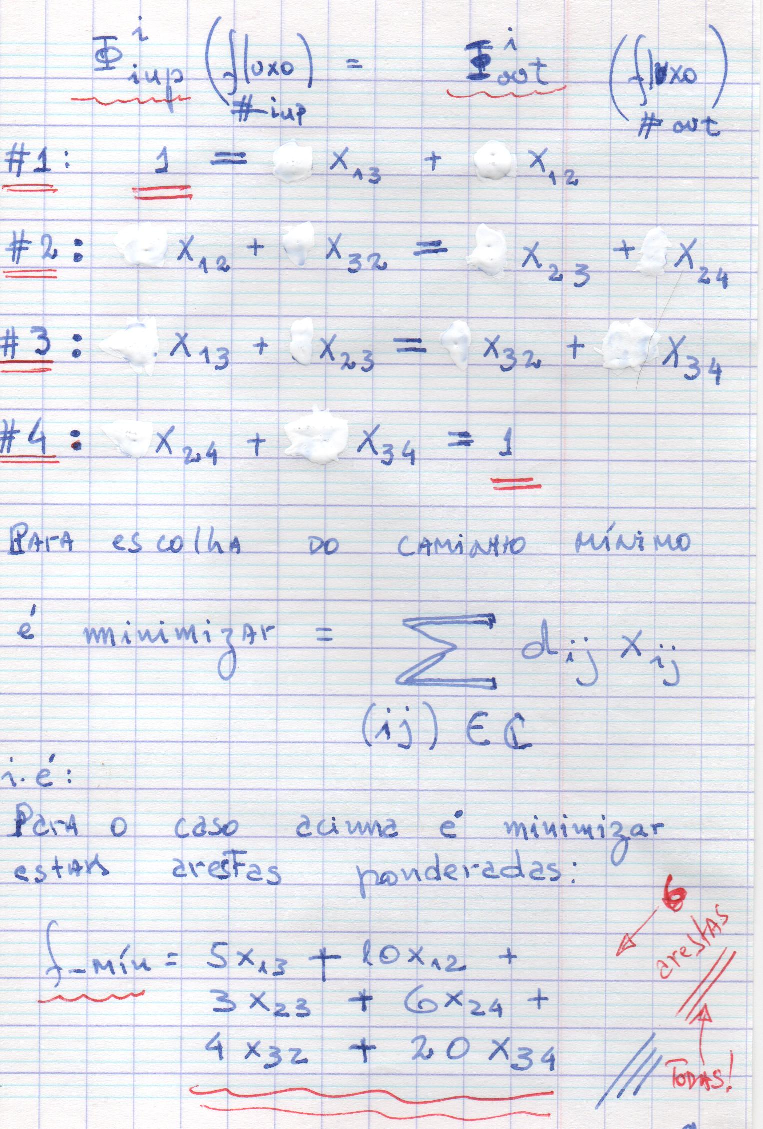
\includegraphics[width=0.8\textwidth , height=0.8\textheight]{09_equacoes_finais.pdf}
		\centering
	\end{figure}
\end{frame}
%%%%%%%%%%%%%%%%%%%%%%%%%%%%%%%%%%%%%%%%%%%%%%%%%%%%%%%

\section{Próximos Passos}

\begin{frame} 
	\frametitle{Próximos Passos:}
	
\begin{block}{}
	
	\begin{itemize}
		\item Implementar na OR-TOOLS  com Python (próximo vídeo)
		\item Ferramenta livre mantida pela Google
		\item Suporta várias linguagens de \textit{front-end}: C++, C\#, Java e Python
		\item Vários \textit{solvers}
		\item Vamos usar o {\em solver}: CP-SAT
		\item CP: \textit{Constraint Programming}
				
		\item \textit{Obrigado!}
		
	\end{itemize}
\end{block}
\end{frame}



%%%%%%%%%%%%%%%%%%%%%%%%%%%%%%%%%%%%%%%%%%%%%%%%%%%%
\section*{Contato}

\begin{frame}
\frametitle{Contato e Comentários:}
  
\begin{block}{}
  % Keep the summary *very short*.
  \begin{itemize}
  \item \url{https://claudiocesar.wordpress.com/}
   \item \url{https://github.com/claudiosa}
   \item Email: \url{claudio.sa@udesc.br}
    \item Email: \url{ccs1664@gmail.comr}

  \item \textit{Thank you so much}!

  \end{itemize}
  \end{block}

\end{frame}


%%%%%%%%%%%%%%%%%%%%%%%%%%%%%%%%%%%%%%%%%%%%%%%%%%%%%%%



\end{document}
